\section{Results}
\label{sec:results}

\subsection*{Arrests}

Figure \ref{fig:es_arrests_main} reports CSDID event-study estimates with controls for arrests, pre-trial detention, and releases. The outcome labeled arrests corresponds to the log of total processed individuals in the original data. Across the three outcomes, the pre-treatment estimates are centered near zero, while the post-treatment estimates are generally positive. This pattern indicates that prison openings are associated with a larger flow of individuals through the criminal justice system, rather than only with a mechanical increase in detention.

\begin{figure}[!htpb]
    \centering
    \caption{Dynamic effects of prison openings on arrests}
    \label{fig:es_arrests_main}
    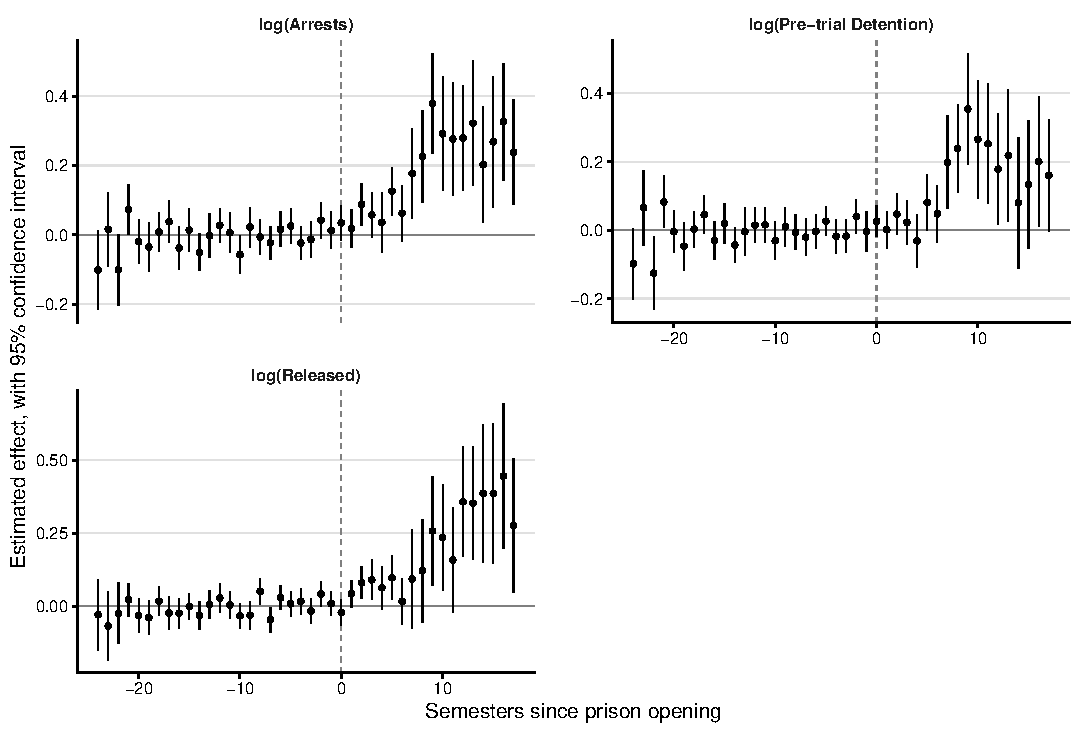
\includegraphics[width=\textwidth]{../results/figures/final_paper/es_arrests_main.pdf}
    \begin{minipage}{0.95\textwidth}
    \footnotesize \emph{Notes:} The figure reports CSDID event-study estimates with controls. Points denote dynamic treatment effects and vertical bars report 95 percent confidence intervals. The outcome labeled ``Arrests'' corresponds to the log of total processed individuals in the original data.
    \end{minipage}
\end{figure}

Table \ref{tab:att_arrests} summarizes the corresponding average effects. With controls, prison openings increase log arrests by 0.096, log pre-trial detention by 0.059, and log releases by 0.090. The positive estimate for releases is important because it helps distinguish a pure detention-capacity story from a broader increase in case processing. The estimates therefore suggest that additional prison capacity is associated with more arrests and more first-hearing decisions overall, not necessarily with more crime.

\begin{table}[!htpb]\centering
\caption{Average treatment effects on arrests}
\label{tab:att_arrests}
\scriptsize
\begin{threeparttable}
\begin{tabular}{@{\extracolsep{0pt}}lccc}
\hline\hline
 & \shortstack{log\\(Arrests)} & \shortstack{log\\(Pre-trial\\ Detention)} & \shortstack{log\\(Released)} \\
 & (1) & (2) & (3) \\
\hline
ATT, no controls & 0.084 & 0.069 & 0.056 \\
 & [0.024] & [0.024] & [0.021] \\
ATT, with controls & 0.096 & 0.059 & 0.090 \\
 & [0.027] & [0.027] & [0.030] \\
Controls & Yes & Yes & Yes \\
Observations & 63,882 & 63,882 & 63,882 \\
Pure control mean & 1.392 & 1.283 & 0.474 \\
\hline\hline
\end{tabular}
\begin{tablenotes}[flushleft]
\item \emph{Notes:} The table reports CSDID average treatment effects. Standard errors clustered by municipality are in brackets. Outcomes are transformed using \(\log(1+y)\). The outcome labeled Arrests corresponds to total processed individuals in the original data.
\end{tablenotes}
\end{threeparttable}
\end{table}



\subsection*{Sentencing outcomes}

The sentencing results examine the extensive margin of sentencing, the type of sentence, and the intensity of punishment. Figure \ref{fig:es_sentencing_decisions} reports event-study estimates for total sentenced individuals, guilty verdicts with prison sentences, guilty verdicts with monetary sentences, and not-guilty decisions. The post-treatment estimates are positive for total sentenced individuals and prison sentences, while the estimates for monetary sentences and not-guilty decisions are less stable and generally less precise.

\begin{figure}[!htpb]
    \centering
    \caption{Dynamic effects of prison openings on sentencing decisions}
    \label{fig:es_sentencing_decisions}
    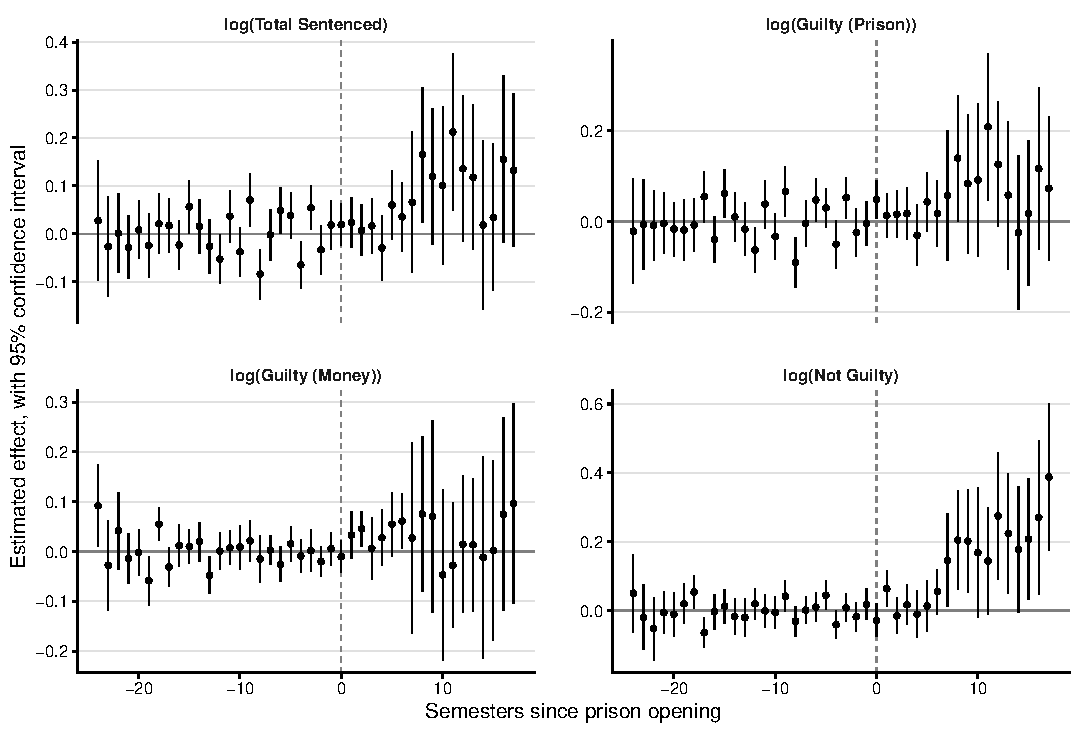
\includegraphics[width=\textwidth]{../results/figures/final_paper/es_sentencing_decisions.pdf}
    \begin{minipage}{0.95\textwidth}
    \footnotesize \emph{Notes:} The figure reports CSDID event-study estimates with controls. Points denote dynamic treatment effects and vertical bars report 95 percent confidence intervals. Count outcomes are transformed using \(\log(1+y)\).
    \end{minipage}
\end{figure}

Figure \ref{fig:es_sentence_length} separately reports sentence-length outcomes. The first panel uses average sentence length, while the second uses \(\log(1+\text{sentence length})\), which keeps zero sentence lengths defined. These estimates are noisy and do not provide strong evidence that prison openings increased the intensity of punishment conditional on reaching the sentencing stage.

\begin{figure}[!htpb]
    \centering
    \caption{Dynamic effects of prison openings on sentence length}
    \label{fig:es_sentence_length}
    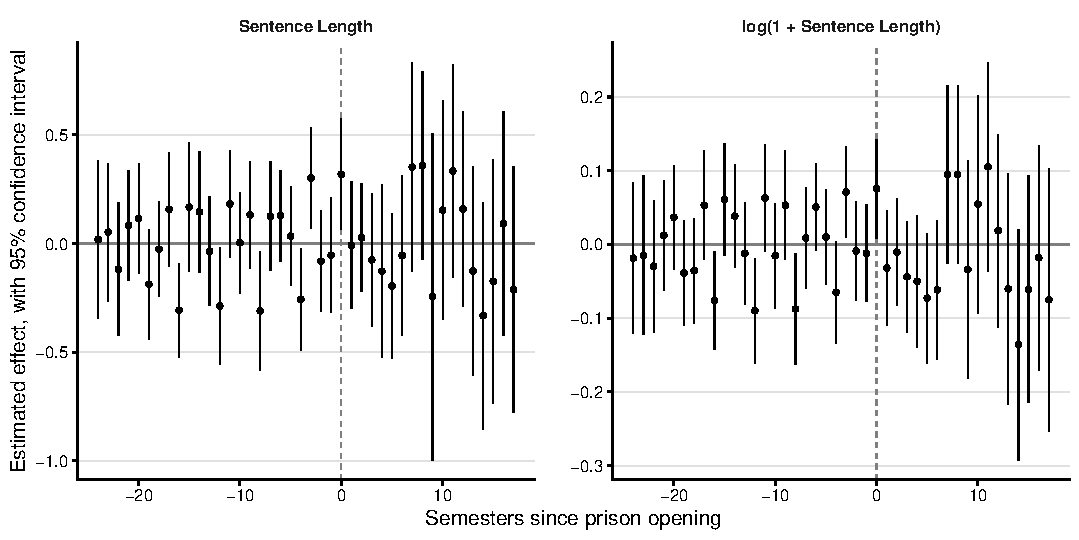
\includegraphics[width=\textwidth]{../results/figures/final_paper/es_sentence_length.pdf}
    \begin{minipage}{0.95\textwidth}
    \footnotesize \emph{Notes:} The figure reports CSDID event-study estimates with controls. Points denote dynamic treatment effects and vertical bars report 95 percent confidence intervals. Sentence Length is the average sentence length among sentenced individuals; the log specification uses \(\log(1+y)\).
    \end{minipage}
\end{figure}

Table \ref{tab:att_sentencing} shows a similar pattern. With controls, the estimated effects are 0.035 for log total sentenced and 0.031 for log guilty prison sentences. The estimates for log guilty monetary sentences and log not-guilty decisions are positive but imprecise, and the estimates for sentence length are close to zero. Overall, the sentencing evidence is most consistent with an increase in the number of cases reaching prison sentences, with weaker evidence of changes in monetary sentences, acquittals, or sentence length.

\begin{table}[!htpb]\centering
\caption{Average treatment effects on sentencing outcomes}
\label{tab:att_sentencing}
\scriptsize
\begin{threeparttable}
\begin{tabular}{@{\extracolsep{0pt}}lcccccc}
\hline\hline
 & \shortstack{log\\(Total\\ Sentenced)} & \shortstack{log\\(Guilty\\ (Prison))} & \shortstack{log\\(Guilty\\ (Money))} & \shortstack{log\\(Not\\ Guilty)} & \shortstack{Sentence\\ Length} & \shortstack{log(1 +\\ Sentence\\ Length)} \\
 & (1) & (2) & (3) & (4) & (5) & (6) \\
\hline
ATT, no controls & 0.036 & 0.039 & -0.018 & 0.030 & 0.106 & 0.017 \\
 & [0.022] & [0.021] & [0.012] & [0.018] & [0.092] & [0.026] \\
ATT, with controls & 0.035 & 0.031 & 0.028 & 0.049 & 0.008 & -0.018 \\
 & [0.025] & [0.022] & [0.024] & [0.025] & [0.118] & [0.031] \\
Controls & Yes & Yes & Yes & Yes & Yes & Yes \\
Observations & 63,882 & 63,882 & 63,882 & 63,882 & 63,882 & 63,882 \\
Pure control mean & 1.132 & 1.029 & 0.109 & 0.428 & 2.131 & 0.818 \\
\hline\hline
\end{tabular}
\begin{tablenotes}[flushleft]
\item \emph{Notes:} The table reports CSDID average treatment effects. Standard errors clustered by municipality are in brackets. Count outcomes are transformed using \(\log(1+y)\). Sentence Length is the average sentence length among sentenced individuals, with zeros assigned when no individuals are sentenced in a municipality-semester.
\end{tablenotes}
\end{threeparttable}
\end{table}



Two points deserve emphasis. First, the interpretation in this section relies on CSDID estimates with controls. Second, the similarity between CSDID estimates with and without controls in Tables \ref{tab:att_arrests} and \ref{tab:att_sentencing} strengthens the case that the results are not driven by the included baseline covariates.

\subsection*{Identifying assumptions}

As discussed in the previous section, identifying the Average Treatment on the Treated (ATT) effects of federal prison construction on local sentencing outcomes does not require assuming that the timing or location of prison construction was random. Instead, identification relies on a weaker parallel trends assumption: in the absence of prison construction, municipalities located near new facilities would have exhibited similar incarceration trends as those farther away. Although this assumption is inherently untestable, I provide substantial empirical evidence supporting its plausibility.

One potential concern is that the executive branch strategically chose the timing and location of federal prison construction in response to pre-existing trends in local prison capacity. Under this alternative explanation, federal prisons would have been built precisely in areas where state-level prisons were becoming increasingly overcrowded, in order to alleviate local capacity pressures. I address this concern in two ways. First, as documented earlier, the 2009 decision to construct private federal prisons was publicly justified by President Felipe Calderón as part of a nationwide effort to relocate individuals convicted of federal crimes into federal facilities, since many were being housed in state prisons. This rationale suggests that the policy was driven by jurisdictional considerations rather than by localized trends in state prison overcrowding. The problem was not uneven local congestion, but rather insufficient federal infrastructure to comply with existing legal mandates.

Second, if prison construction had been systematically targeted toward areas experiencing worsening local overcrowding, we would expect to observe differential pre-treatment trends in overcrowding between treated and control municipalities. Figures \ref{fig:capacity} and \ref{fig:capacity_robust} show no evidence of such pre-trends in relative overcrowding at the local level, providing direct evidence against this selection mechanism.

A related concern is that the executive—particularly under President Felipe Calderón—may have strategically directed prison construction toward regions experiencing rising crime or intensified enforcement. The War on Drugs was publicly launched in Michoacán with the deployment of the army on December 11, 2006. However, Table \ref{tab:app1tab} shows that the federal prison in Michoacán was not completed until 2016. In contrast, the federal prisons built after the start of the war—whose construction likely began during the early years of the conflict—were located in the Southeast (Veracruz and Tabasco), while Michoacán is in the West. This pattern suggests that the crackdowns were not accompanied by contemporaneous increases in federal incarceration capacity in the regions most affected by the initial enforcement efforts. Moreover, if this were the case, we would expect to observe differential pre-treatment trends in criminal justice activity, such as arrests. Figure \ref{fig:es_arrests_main} shows no such systematic pre-trends, further supporting the validity of the parallel trends assumption.

\subsection*{Mechanisms}

The main results show increases in arrests and in some sentencing outcomes. I next examine whether the composition of these increases is consistent with a broad rise in serious crime or with greater processing of lower-level cases and more vulnerable defendants.

\subsubsection*{Arrests by type of crime}

Figure \ref{fig:es_crime_type_main} reports event-study estimates for selected crime categories. The clearest positive dynamics are for property crimes and bodily injury and physical harm. Homicides are much flatter, while weapons offenses do not show a comparable increase. This composition is consistent with the interpretation that expanded prison capacity increased enforcement or processing primarily for lower-level offenses, rather than reflecting an increase in serious violent crime.

\begin{figure}[!htpb]
    \centering
    \caption{Dynamic effects of prison openings on arrests by type of crime}
    \label{fig:es_crime_type_main}
    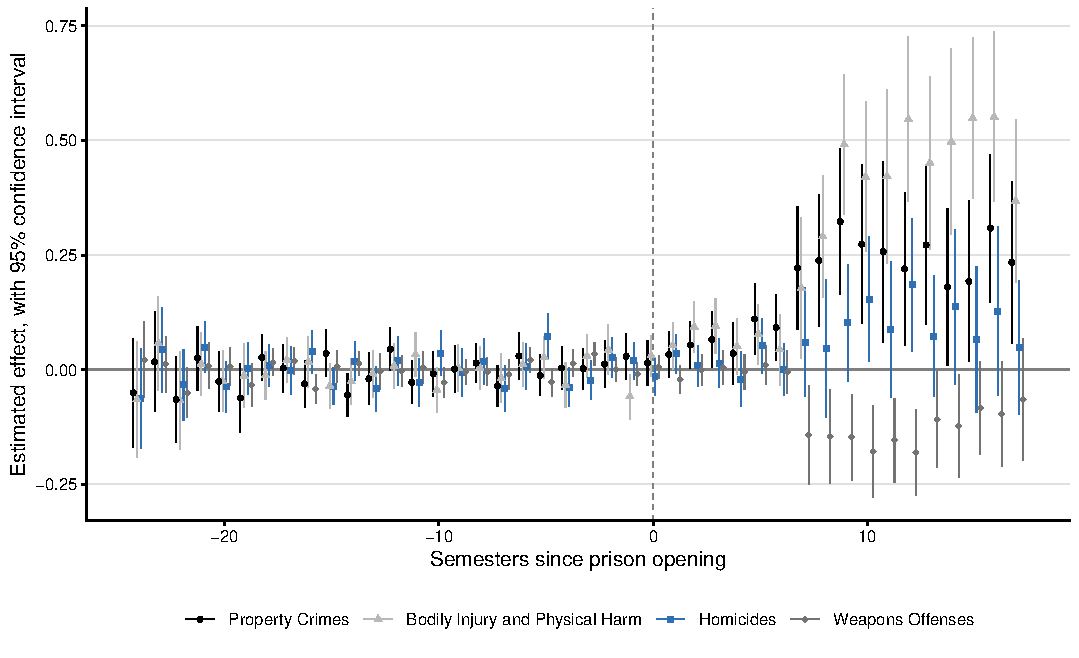
\includegraphics[width=\textwidth]{../results/figures/final_paper/es_crime_type_main.pdf}
    \begin{minipage}{0.95\textwidth}
    \footnotesize \emph{Notes:} The figure reports CSDID event-study estimates with controls. Points denote dynamic treatment effects and vertical bars report 95 percent confidence intervals. Outcomes are crime-category arrest counts transformed using \(\log(1+y)\).
    \end{minipage}
\end{figure}

Table \ref{tab:att_crime_type} reports the average effects for all available crime categories. The largest estimates are for bodily injury and physical harm (0.128) and property crimes (0.088). By contrast, the estimates for homicides (0.025), drugs (-0.018), and weapons offenses (-0.025) are small or negative. The pattern suggests that the increase in arrests is concentrated in lower-level categories and not in the most serious violent or federalized categories.

\begin{table}[!htpb]\centering
\caption{Average treatment effects on arrests by type of crime}
\label{tab:att_crime_type}
\scriptsize
\begin{threeparttable}
\begin{adjustbox}{max width=\textwidth}
\begin{tabular}{@{\extracolsep{0pt}}lccccccccccc}
\hline\hline
 & \shortstack{Property\\ Crimes} & \shortstack{Bodily\\ Injury\\ and\\ Physical\\ Harm} & \shortstack{Homicides} & \shortstack{Drugs} & \shortstack{Guns} & \shortstack{Kidnapping\\ and\\ Personal\\ Liberty} & \shortstack{Sexual\\ Liberty\\ and\\ Security} & \shortstack{Family\\ and\\ Domestic\\ Violence} & \shortstack{Other\\ Public\\ Health\\ Offenses} & \shortstack{Public\\ Administration\\ Offenses} & \shortstack{Threats\\ and\\ Other\\ Legal\\ Interests} \\
 & (1) & (2) & (3) & (4) & (5) & (6) & (7) & (8) & (9) & (10) & (11) \\
\hline
Effect of federal prison construction, with controls & 0.088 & 0.128 & 0.025 & -0.018 & -0.025 & -0.004 & 0.036 & 0.024 & 0.028 & 0.049 & 0.026 \\
 & [0.026] & [0.025] & [0.021] & [0.022] & [0.016] & [0.016] & [0.020] & [0.026] & [0.009] & [0.025] & [0.020] \\
Controls & Yes & Yes & Yes & Yes & Yes & Yes & Yes & Yes & Yes & Yes & Yes \\
Observations & 63,882 & 63,882 & 63,882 & 63,882 & 63,882 & 63,882 & 63,882 & 63,882 & 63,882 & 63,882 & 63,882 \\
Pure control mean & 0.930 & 0.698 & 0.382 & 0.060 & 0.247 & 0.061 & 0.389 & 0.376 & 0.010 & 0.259 & 0.199 \\
\hline\hline
\end{tabular}
\end{adjustbox}
\begin{tablenotes}[flushleft]
\item \emph{Notes:} The table reports CSDID average treatment effects with controls. Standard errors clustered by municipality are in brackets. Outcomes are counts by crime category transformed using \(\log(1+y)\). The treatment variable is an indicator for federal prison construction within 300KM of a municipality. CSDID controls are PMASC18\_, VP\_TV, VP\_RADIO, and PNOTRABA.
\end{tablenotes}
\end{threeparttable}
\end{table}



\subsubsection*{Arrests of marginalized individuals}

The available mechanism data also identify cases involving marginal-condition defendants. Figure \ref{fig:es_marginalized_status} compares marginal-condition cases with non-marginal-condition cases, defined as the total minus marginal-condition cases before applying the log transformation. The figure separates arrests and pre-trial detention into panels and overlays the two defendant groups within each panel. The estimates are best interpreted as evidence on composition: both groups show positive post-treatment effects, but the increase is larger for marginal-condition defendants. This suggests that the increase in arrests includes more socially vulnerable defendants, although the available data do not separately identify every socioeconomic category discussed in the descriptive section.

\begin{figure}[!htpb]
    \centering
    \caption{Dynamic effects of prison openings by defendant marginal condition}
    \label{fig:es_marginalized_status}
    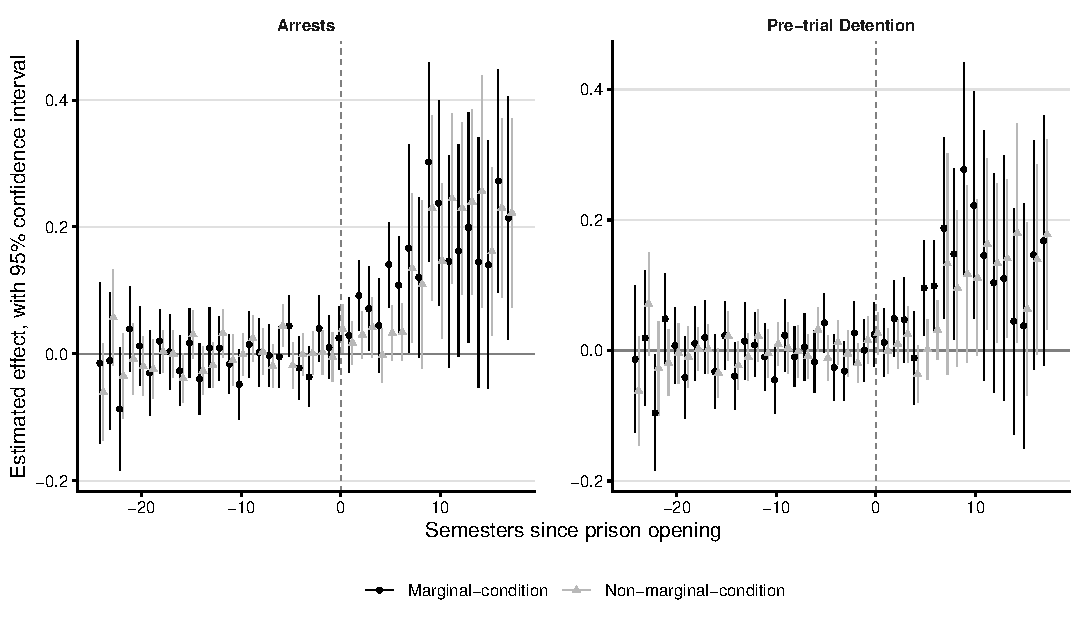
\includegraphics[width=\textwidth]{../results/figures/final_paper/es_marginalized_status.pdf}
    \begin{minipage}{0.95\textwidth}
    \footnotesize \emph{Notes:} The figure reports CSDID event-study estimates with controls. Points denote dynamic treatment effects and vertical bars report 95 percent confidence intervals. Outcomes are transformed using \(\log(1+y)\). Non-marginal-condition arrests are total arrests minus marginal-condition arrests before transformation. Non-marginal-condition pre-trial detention is total pre-trial detention minus marginal-condition pre-trial detention before transformation.
    \end{minipage}
\end{figure}

Table \ref{tab:att_marginalized} reports the corresponding average effects. The estimate for marginal-condition arrests is 0.091, compared with 0.069 for non-marginal-condition arrests. For pre-trial detention, the estimate is 0.061 for marginal-condition defendants and 0.043 for non-marginal-condition defendants. This pattern is consistent with the interpretation that the additional processing includes socially vulnerable defendants and is somewhat more pronounced among them.

\begin{table}[!htpb]\centering
\caption{Average treatment effects by defendant socioeconomic status}
\label{tab:att_marginalized}
\scriptsize
\begin{threeparttable}
\begin{tabular}{@{\extracolsep{0pt}}lcccc}
\hline\hline
 & \shortstack{Marginal-condition\\ arrests} & \shortstack{Non-marginal-condition\\ arrests} & \shortstack{Marginal-condition\\ pre-trial detention} & \shortstack{Non-marginal-condition\\ pre-trial detention} \\
 & (1) & (2) & (3) & (4) \\
\hline
Effect of federal prison construction & 0.091 & 0.059 & 0.061 & 0.031 \\
 & [0.028] & [0.022] & [0.027] & [0.021] \\
Controls & Yes & Yes & Yes & Yes \\
Observations & 63,882 & 63,882 & 63,882 & 63,882 \\
Pure control mean & 1.131 & 0.284 & 1.049 & 0.247 \\
\hline\hline
\end{tabular}
\begin{minipage}{0.95\textwidth}
\footnotesize \emph{Notes:} The table reports CSDID average treatment effects with controls. Standard errors clustered by municipality are in brackets. Outcomes are transformed using \(\log(1+y)\). Non-marginal-condition outcomes use the non-marginalized variables from the interaction datasets. The treatment variable is an indicator for federal prison construction within 300KM of a municipality. Estimates use CSDID with controls.
\end{minipage}
\end{threeparttable}
\end{table}



\subsubsection*{Sentencing by sentence-length category}

Finally, I examine whether the sentencing increase is concentrated in short-sentence categories. Figure \ref{fig:es_sentence_categories_main} compares the two shortest sentence-length categories with the highest sentence-length category. The dynamics are more positive for the short-sentence categories, especially the one-to-twelve-month category, and much flatter for sentences of twenty-one years or more.

\begin{figure}[!htpb]
    \centering
    \caption{Dynamic effects of prison openings by sentence-length category}
    \label{fig:es_sentence_categories_main}
    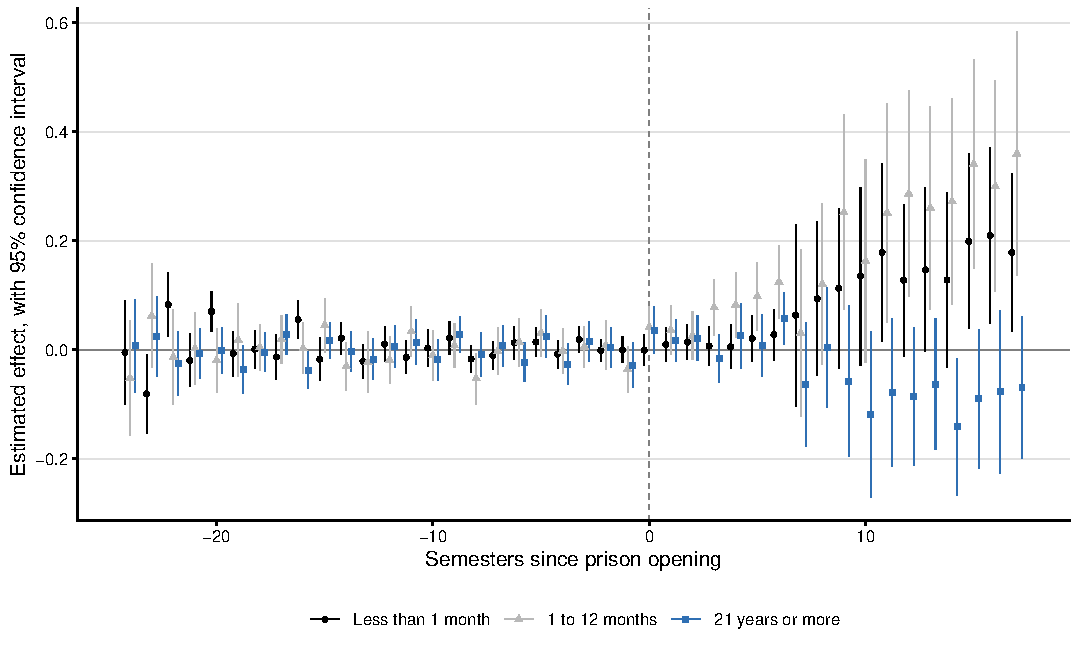
\includegraphics[width=\textwidth]{../results/figures/final_paper/es_sentence_categories_main.pdf}
    \begin{minipage}{0.95\textwidth}
    \footnotesize \emph{Notes:} The figure reports CSDID event-study estimates with controls. Points denote dynamic treatment effects and vertical bars report 95 percent confidence intervals. Outcomes are counts of sentenced individuals in each sentence-length category, transformed using \(\log(1+y)\).
    \end{minipage}
\end{figure}

Table \ref{tab:att_sentence_categories} reports all sentence-length categories. The largest estimate is for sentences of one to twelve months (0.096), while estimates for longer sentence categories are smaller, close to zero, or imprecise. This sentencing composition is consistent with an increase in the processing of petty or lower-level offenses, rather than a broad increase in serious criminal convictions.

\begin{table}[!htpb]\centering
\caption{Average treatment effects by sentence-length category}
\label{tab:att_sentence_categories}
\scriptsize
\begin{threeparttable}
\begin{adjustbox}{max width=\textwidth}
\begin{tabular}{@{\extracolsep{0pt}}lccccccccccccc}
\hline\hline
 & \shortstack{Less\\ than\\ 1\\ month} & \shortstack{1\\ to\\ 12\\ months} & \shortstack{1\\ to\\ 3\\ years} & \shortstack{3\\ to\\ 5\\ years} & \shortstack{5\\ to\\ 7\\ years} & \shortstack{7\\ to\\ 9\\ years} & \shortstack{9\\ to\\ 11\\ years} & \shortstack{11\\ to\\ 13\\ years} & \shortstack{13\\ to\\ 15\\ years} & \shortstack{15\\ to\\ 17\\ years} & \shortstack{17\\ to\\ 19\\ years} & \shortstack{19\\ to\\ 21\\ years} & \shortstack{21\\ years\\ or\\ more} \\
 & (1) & (2) & (3) & (4) & (5) & (6) & (7) & (8) & (9) & (10) & (11) & (12) & (13) \\
\hline
Effect of federal prison construction, with controls & 0.034 & 0.096 & -0.022 & -0.001 & -0.008 & 0.017 & 0.034 & 0.004 & 0.007 & 0.018 & -0.004 & 0.013 & 0.004 \\
 & [0.021] & [0.023] & [0.026] & [0.019] & [0.022] & [0.019] & [0.015] & [0.013] & [0.015] & [0.012] & [0.008] & [0.013] & [0.019] \\
Controls & Yes & Yes & Yes & Yes & Yes & Yes & Yes & Yes & Yes & Yes & Yes & Yes & Yes \\
Observations & 63,882 & 63,882 & 63,882 & 63,882 & 63,882 & 63,882 & 63,882 & 63,882 & 63,882 & 63,882 & 63,882 & 63,882 & 63,882 \\
Pure control mean & 0.092 & 0.519 & 0.541 & 0.354 & 0.191 & 0.138 & 0.112 & 0.091 & 0.055 & 0.053 & 0.030 & 0.037 & 0.163 \\
\hline\hline
\end{tabular}
\end{adjustbox}
\begin{tablenotes}[flushleft]
\item \emph{Notes:} The table reports CSDID average treatment effects with controls. Standard errors clustered by municipality are in brackets. Outcomes are counts of sentenced individuals in each sentence-length category, transformed using \(\log(1+y)\). The treatment variable is an indicator for federal prison construction within 300KM of a municipality. CSDID controls are PMASC18\_, VP\_TV, VP\_RADIO, and PNOTRABA.
\end{tablenotes}
\end{threeparttable}
\end{table}



\subsection*{Robustness checks}

\subsubsection*{Robustness to other HTE methods}

Figures \ref{fig:att_first_robust} and \ref{fig:att_sent_robustness} present the main results using alternative estimators: \cite{Borusyak-DIDImp} (didimputation) and \cite{SunAb} (SunAb). Across all dependent variables in levels, the ATT estimates are statistically indistinguishable, with closely aligned point estimates. The \cite{SunAb} estimator is effectively equivalent to \cite{Callaway} without controls, since both rely on 2x2 group comparisons across groups (excluding forbidden comparisons, such as using treated units as controls). The motivation for including an imputation-based method lies in its efficiency under homoskedasticity, as demonstrated by \cite{Borusyak-DIDImp}. Although some degree of serial correlation across units is likely, efficiency gains are still expected even under low correlation \citep{Chaise-ReviewDID}. In line with these theoretical results, imputation-based estimates prove more efficient than the event-by-event HTE-robust methods.

The robustness checks require careful interpretation. In general, results are consistent across specifications, but not uniformly across all variables. For instance, rate-based variables yield differences across estimators: the rate of pre-trial detention to arrests displays a sign change and significance only with the imputation method. This likely reflects two issues—first, the need to impute zeros for municipalities without cases and include controls for this, and second, the possibility that the denominator itself is affected by the treatment. 

Moreover, in some cases, efficiency gains from imputation methods transform similar point estimates into statistically significant results. Three variables deserve special attention: the rate of pre-trial detention to arrests, the log of individuals sentenced not guilty, and sentencing length. To examine these, I plot event-study estimates using \cite{Gardner} and \cite{Liu-FECT} together with \cite{Borusyak-DIDImp}. For sentencing length, Figure \ref{fig:sent_intensive_event_robust} shows post-treatment patterns that look similar across methods, with a clear increase after prison construction. The imputation methods estimate this more precisely, making the ATT significant. The interpretation therefore remains the same: even if ATT estimates differ across methods, the event studies point to a positive post-treatment trend in sentencing length.

The other two variables offer less consistent results. Figures \ref{fig:event_study_absolutoria} and \ref{fig:event_study_pretrial} show that the different methods give different answers. For non-guilty sentences, both sets of methods show a small increase about two years after construction followed by a decline, but the imputation methods make the increase larger and significant, while the event-by-event estimates do not. For the pre-trial detention rate, event-by-event methods suggest a lasting increase, while imputation methods show a negative trend. Because of these differences, it is hard to reach firm conclusions for these two outcomes. 

\subsubsection*{Robustness to transformations of the dependent variable}
\label{sec:robust_log}
As noted in the main results, all models for variables in levels are estimated using a log transformation of the dependent variable. This choice makes treatment effects easier to interpret as percentage changes. It also helps address skewness in the data: the number of arrests is likely higher in municipalities with larger populations (or other correlated factors), and the log transformation reduces the influence of outliers in the estimation.

However, despite these advantages, \cite{ChenRoth2024} highlight several biases that can arise when using log transformations to estimate treatment effects. These concerns apply not only to ATEs but also to DiD settings (ATTs). The main issue is that in contexts with an extensive margin—where treatment can change an outcome from zero to positive—treatment effects depend on the arbitrary choice of scale. By simply re-scaling the log-transformed dependent variable by a scalar $a$, one could generate any treatment effect. This problem arises because percentage effects are not well defined for observations that move from zero to nonzero after treatment. In such cases, the units of the outcome implicitly determine the weight placed on the extensive margin. In this context, treatment effects are not well defined for municipalities with no arrests or sentenced individuals at time $t$ when their outcomes shift from zero to positive—for example, municipalities that would process no cases without a nearby prison but would process at least one once a new facility is built.

I provide evidence that these theoretical concerns do not bias the main results presented in the previous section. Figure \ref{fig:att_sent_robustness_chen} reports the ATTs for all outcomes in levels estimated with the $log(y+1)$ transformation. Two points are worth highlighting. First, across all variables except one, there is no evidence of an extensive-margin treatment effect ($1\{y>0\}$): ATT estimates are precisely estimated null effects, with the only exception being the not-guilty outcome. Second, results using the hyperbolic sine transformation ($arcsinh(y) = \log(y + \sqrt{1 + y^2})$) closely match those from the log-like specification. Finally, because both $arcsinh(y)$ and $log(y+1)$ suffer from the unit-dependence problem, I also estimate ATTs using the transformation proposed by \cite{ChenRoth2024}, which calibrates the extensive margin by setting $y=0$ to $-x$ (where $x = \min\{y>0\}$) and $\log(y)$ for $y>0$, so that moving from 0 to 1 is interpreted as a 100\% increase. Results remain robust under this specification. 

Also connected to this are the event study results for the levels variables, which show a significant short-term increase followed by a sharp decline in the later periods. Two mechanisms could explain this trend. First, as illustrated in Figure \ref{fig:event_view_300km}, the group of municipalities treated at the earliest stage could have experienced a structural change in the final periods that drove levels downward. The point estimates are highly noisy and largely influenced by these municipalities. At the moment I have not found anything that can explain this, but additional evidence must be studied to discard this. Second, it is possible that municipalities with continuous case activity are driving the observed rise and fall in caseloads. However, this explanation is less convincing, since the extensive margin shows no effect and the same pattern does not appear across all outcomes, particularly those unrelated to prison outcomes. In general, further investigation need to be done, as the pattern is concerning and might be showing a bias on the overall results.

Finally, one additional point is worth noting. In the main results, I raised the possibility that estimates using rate-based dependent variables (e.g., the share of guilty individuals sentenced to prison or the ratio of pre-trial detentions to arrests) could be biased. This arises because imputing zeros for municipalities with a denominator of zero requires adding a control: a dummy variable equal to one when the denominator variable is greater than zero and zero otherwise. The concern is that if treatment also affects the extensive margin, this dummy becomes endogenous to treatment and functions as a bad control. Figure \ref{fig:att_sent_robustness_chen}, however, shows that treatment is not correlated with this extensive-margin dummy for arrests and sentenced cases, alleviating this concern.

\subsubsection*{Robustness to different thresholds}

As specified in Section \ref{sec:emp}, treatment is defined using the minimum distance from each municipality to a federal prison. I adopt a data-driven thresholding approach: the median and mean of this distance are 236 km and 252 km, respectively, so I set the cutoff at 300 km—a round figure and a multiple of 100. This choice is further motivated by anecdotal evidence suggesting that federal prisons were intended to influence broader geographic zones rather than individual municipalities or entire states. Nevertheless, the choice of 300 km remains to some extent arbitrary. To assess the robustness of the results to alternative definitions of treatment, I re-estimate the same specification for the same outcomes using thresholds that vary by increments of +1 km within a +-50 km window around 300 km. Figure \ref{fig:att_sent_robust_thres} shows that both the point estimates and their associated standard errors remain nearly unchanged across these 100 alternative treatment definitions, providing strong evidence that the findings are robust to threshold selection. 

\subsubsection*{ITT and continuous treatment (discussion)}

One institutional feature that motivates the treatment definition is that, under Mexican law, individuals from municipality $x$ are typically assigned to serve their sentence in the nearest federal prison (with the exception of gang-related crimes, which are excluded from the analysis). However, because I generally do not observe the actual prison to which each individual was assigned, the estimated effect might not be the average treatment effect on the treated (ATT), which is what generally is estimated using DiD. Rather, it more closely resembles an intent-to-treat (ITT) effect: what I identify is the effect of being in a municipality located within the area covered by a federal prison, regardless of whether all individuals from that municipality were actually sent there. However, since the analysis is aggregated at the municipality level, an argument could be made to interpret the effects as increases in the probability of being sentenced to prison, given that your municipality is on the vicinity of a newly constructed prison.

A further assumption, related to this and to the previous section, is that treatment is binary—once a prison is constructed within a given threshold distance of a municipality I assign 1, 0 otherwise. This definition rests on two implicit assumptions. First, once a prison is built within the defined vicinity, municipalities just inside the threshold are assumed to be affected in the same way as those located directly adjacent to the prison. This assumption is plausible in light of the institutional context, and is reinforced by the argument that prison construction alleviates overcrowding at the state level; in practice, zones rather than individual municipalities are the affected units, this affected units are determined by distance to the center rather than borders (states) or demarcations, so the precise distance within the zone may matter less once the threshold is crossed.

The second assumption is that municipalities are not additionally affected if a second or third prison is constructed closer than the first. This assumption is less plausible, since the capacity channel would suggest that successive increases in capacity should yield additional effects. Nonetheless, for tractability, treatment is modeled as binary rather than continuous.

Ideally, treatment would instead be defined continuously, capturing the effect of reducing the distance to the nearest federal prison. This motivates the following alternative specification:

\begin{equation}
\label{eq:eq4}
    Y_{pt} = \phi + \beta \, DistanceInv_{pt} + \gamma_t + \tau_p + \epsilon_{pt},
\end{equation}

where $DistanceInv_{pt}$ is defined as
\begin{equation}
\label{eq:eq5}
DistanceInv_{pt} =
\begin{cases}
0, & \text{if } MinDistance_{pt} > Threshold, \\
\dfrac{MinDistance_{pt} - Threshold}{Threshold}, & \text{if } MinDistance_{pt} \leq Threshold,
\end{cases}
\end{equation}

with $MinDistance_{pt}$ denoting the minimum distance from municipality $p$ to the closest federal prison at time $t$. Recent literature on generalized difference-in-differences (DiD) designs has highlighted some challenges in correctly identifying unbiased effects when using a continuous treatment \citep{Cont-Chaise-AEA, CallawayGoodmanBaconSantAnna2024}. First and foremost, for correct interpretation of the effects, a stronger parallel trends assumption has to hold, which is that the trajectory of outcomes for lower-dose units must represent how the outcomes of higher-dose units would have evolved had they been exposed to the lower dose instead \citep{CallawayGoodmanBaconSantAnna2024}.

Unfortunately, none of these estimators can be applied to the context in hand. \cite{CallawayGoodmanBaconSantAnna2024} requires that the continuous treatment is absorbing, meaning that once it goes from 0 to a dose $d>0$, it has to stay in that level till the end of the study period. In my context, the continuous variable would increase once the distance to a federal prison decreases over time (when new prisons are built closer). \cite{Cont-Chaise-AEA} assumes that there are no stayers, meaning that all units change from period $t-1$ to period $t$ to a different dose. In my case, some units will remain at the same distance to a prison at different points in time. 

One important caveat is that there are concerns with using this specification, even if it were unbiased. First, constructing the treatment as a continuous variable would make the resulting coefficient difficult to interpret. At best, the interpretation would reduce to a relative measure of proximity on a 0–1 scale: municipalities with values closer to 1 are nearer to a federal prison. This interpretability issue does not arise with the current binary specification. Moreover, adopting a continuous treatment would make the parallel trends assumption considerably more difficult to satisfy, as it would need to hold across the group with low doses and the groups with high, rather than only between treated and untreated groups. Even with these concerns, adding this analysis is considered for future steps.
